\documentclass{article}
\usepackage[english]{babel}
\usepackage[utf8]{inputenc}
\usepackage{lpic}
\usepackage[usenames,dvipsnames]{xcolor}
\usepackage{punk}
\usepackage[T1]{fontenc}
\pagestyle{empty}
\usepackage{tikz}
\usepackage[papersize={12.709408in,9.250in}, spine=0.459508in, cropgap=0.125in
,cropmarks, cropframe
]{zwpagelayout}
\linespread{1}
\definecolor{orange}{RGB}{250,205,25}
\pagecolor{orange}
\begin{document}
\begin{lpic}[t(5in),b(0mm),r(0mm),l(7.5in)]{lambert-bug(1)}
\lbl[b]{17,105;{\hbox{
\hspace{3em}\parbox{.3\textwidth}{\punkfamily\bfseries\Huge  Euclidean Plane and its Relatives}}}}
\lbl{23,95;{\punkfamily\LARGE A minimalistic introduction}}
\lbl{23,85;{\punkfamily\large Anton Petrunin}}
\lbl[]{-59,113,-90;{\punkfamily\bfseries\LARGE  Euclidean Plane and its Relatives}}
\lbl{-59,-5,-90;{\punkfamily\large Anton Petrunin}}
\lbl{23,-5;{\punkfamily\large Edition \# 0.2,
for friends only.}}
\lbl{-150,100;{\hbox{
\hspace{3em}\parbox{.3\textwidth}
{\punkfamily\large 
This book is designed for a semester-long course 
in Euclidean and non-Euclidean plane geometries 
and their development from postulate systems. 
We use so called metric approach introduced by Birkhoff.
The lectures are meant to be rigorous, conservative, elementary and minimalistic.}}}}
\lbl{-59.4,32,90;{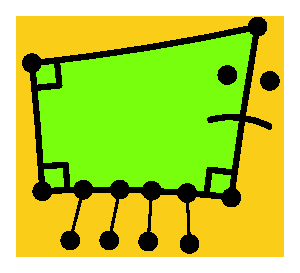
\includegraphics[scale=0.20]{lambert-bug-2}}}
\end{lpic}
\end{document}